\section{Prior Work}

MUIFOLD builds upon a rich body of research done both in
various smartphone-based interaction paradigms, as well as frameworks
for building such applications.

One method that has been used to support remote interactions between a smartphone and a large display is to use the
phone's camera to ``point'' at the screen and interact with
content~\cite{boring_touch_2010,jeon_interaction_2010}. In these
systems, a live video is captured of the display and mirrored onto
the smartphone, which provides the user with a
so-called ``Smart Lens'' onto the screen. Liu et al.~\cite{liu_effects_2014} demonstrated the effectiveness of using a
mobile device as a trackpad for large
displays. Babic et al.~\cite{babic_simo_2020} developed a system, Simo, that tracks a user's gaze onto a screen through the
front and back cameras of a phone. In our own experience, such approaches suffer from a serious drawback. Requiring users to stare through their phone's camera to view content on the large display draws their attention away from their human partners, thereby actually harming the collaboration that the technology is intended to enhance.

Another popular method of interaction is to enable users control a cursor on the
screen~\cite{boring_scroll_2009} or scroll a
page~\cite{oakley_tilt_2005} by tilting their smartphone. Seifert et al. demonstrate using ray-casting to project a cursor onto a display. Unfortunately,
their setup is non-trivial to replicate due to the need for
additional hardware attached to the phone and sensors on the
screen~\cite{hutchison_pointerphone:_2013}. Alternatively,
Pietroszek et al. utilize the built-in sensors of the phone in a
native application to develop the Smartcasting system, which
allows for similar pointing gestures without the need for
additional setup or hardware~\cite{pietroszek_smartcasting:_2014}.
Dingler et al. demonstrate  similar capacity via
a web-based application in their uCanvas system; a limitation is that users cannot move once the system is
calibrated~\cite{abascal_ucanvas_2015}. MUIFOLD is similar to uCanvas in that it uses a web-based application to enable pointing. However, MUIFOLD has a few relative advantages for users and developers. First, it permits users to move freely about most of the space (although there is a slight reduction in functionality when
users stand at a sharp angle to the screen off to the side or
interact with content at either extreme of the screen). As will be detailed in section~\ref{sec:muifold}, MUIFOLD
achieves this through filtering techniques and by allowing users to customize the pixel change per degree of rotation. Second, MUIFOLD
content developers don't need to write any special code to support common functions such as clicking or scrolling.

\begin{figure}
\centering
  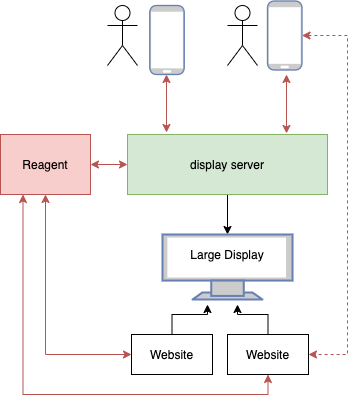
\includegraphics[width=0.6\columnwidth]{chapters/03_muifold/figures/muifold_architecture.png}
  \caption{Architecture of MUIFOLD. The red lines are WebSockets and the dotted line indicates an optional Web Socket depending on application needs.}
  \label{fig:architecture_muifold}
\end{figure}

Among the prior work on building web frameworks for remote interaction between smartphones and large displays is that of
Weißker et al., who proposed a
framework for building out real-time game applications ~\cite{weisker_massive_2016}. Baldauf et al. created the ATREUS
platform, which could be used to build remote control based
devices around varying interaction types and degrees of integration
into the platform by developers~\cite{baldauf_your_2016}. Barsotti
et al. developed the CDI framework, in which developers wrap event listeners around content displayed on a webpage
that is triggered by the smartphone~\cite{barsotti_web_2017}.
In each of these frameworks, users open webpages on their phone that communicate with the display and application via WebSockets.
Both Weißker et al. and Baldauf et al. demonstrated their
work in the context of a game, thereby showing that
WebSockets meet sufficiently stringent low-latency requirements, prompting us to use the same approach for MUIFOLD.

In all three of these prior efforts, application
developers must fully develop the content they wish to show with bindings to the client application running on the smartphone. This prevents the use of arbitrary third-party content on the fly.
All of these authors acknowledged a desire for a technology that would obviate the need for users to download and install a native application tailored to a particular system, such that they could just walk up to it and use it immediately. Through its unique design, MUIFOLD satisfies this desire, and makes it possible for arbitrary sites to ``just work'', while still supporting richer interactions for custom applications if needed.
